\section{Question 4}

\textbf{\textit{Calculate the weighted standardised level difference (D\textsubscript{nT,w}) between the conference room and single office for voice transmission through both the ductwork and the common partition, and discuss the results in terms of privacy.}}


The resolution of D\textsubscript{nT,w} between the conference room and single office for voice transmission through both the ductwork and the common partition is explained in Sections~\ref{sec:Q4.1} to \ref{sec:Q4.3}.
Section~\ref{sec:Q4.4} briefly discusses the results in terms of privacy.



\subsection{Step 1: Calculate D\textsubscript{nT}} \label{sec:Q4.1}

The first step is to calculate the standardised level difference, D\textsubscript{nT}, through the ductwork, through the partition, and through both the ductwork and the partition.
This is done using Equation~\ref{eq:DnT}.
Table~\ref{tbl:DnT_example} details the D\textsubscript{nT} calculations at 63~Hz.
Table~\ref{tbl:DnT} and Figure~\ref{fig:DnT} present the D\textsubscript{nT} results in octave bands between 63~Hz and 4~kHz.

	\begin{equation}\label{eq:DnT}
		D_{nT} = L_1 - L_2 + 10 log \frac{T_2}{0.5}
	\end{equation}

% Please add the following required packages to your document preamble:
% \usepackage{booktabs}
\begin{sidewaystable}[htbp]
	\caption{Details of the calculation of the DnT between the conference room and single office for voice transmission through the ductwork and partition at 63~Hz.}
	\label{tbl:DnT_example}
	\centering
	\begin{tabular}{@{}lrl@{}}
		\toprule
		Frequency (Hz) & 63 & Notes \\ \midrule
		L\textsubscript{p\textsubscript{male\textsubscript{1}}} (dB) & 54.11 & From Table~\ref{tbl:SPL_office} \\
		L\textsubscript{p\textsubscript{male\textsubscript{2}duct}} (dB) & 1.26 & From Table~\ref{tbl:SPL_office} \\
		L\textsubscript{p\textsubscript{male\textsubscript{2}ducts}} (dB) & 1.26 + 3 = 4.27 & L\textsubscript{p\textsubscript{male\textsubscript{2}ducts}} = L\textsubscript{p\textsubscript{male\textsubscript{2}duct}} + 3 \\
		L\textsubscript{p\textsubscript{male\textsubscript{2}partition}} (dB) & 31.76 & From Table~\ref{tbl:SPL_office} \\
		L\textsubscript{p\textsubscript{male\textsubscript{2}}} (dB) & 31.77 & From Table~\ref{tbl:SPL_office} \\
		T\textsubscript{2} (s) & 0.47 & From Table~\ref{tbl:reverb_office} \\
		D\textsubscript{nT} through ductwork (dB) & $54.11 - 4.27 + 10 log \left(\frac{0.47}{0.5}\right) = 49.6$ & $D_{nT} = L_{p_{male_1}} - L_{p_{male_2}ducts} + 10 log \left(\frac{T_2}{0.5}\right)$ \\
		D\textsubscript{nT} through partition (dB) & $54.11 - 31.76 + 10 log \left(\frac{0.47}{0.5}\right) = 22.1$ & $D_{nT} = L_{p_{male_1}} - L_{p_{male_2}partition} + 10 log \left(\frac{T_2}{0.5}\right)$ \\
		D\textsubscript{nT} through ductwork and partition (dB) & $54.11 - 31.77 + 10 log \left(\frac{0.47}{0.5}\right) = 22.1$ & $D_{nT} = L_{p_{male_1}} - L_{p_{male_2}} + 10 log \left(\frac{T_2}{0.5}\right)$ \\ \bottomrule
	\end{tabular}
\end{sidewaystable}

% Please add the following required packages to your document preamble:
% \usepackage{booktabs}
\begin{table}[htbp]
	\caption{Calculation of the DnT between the conference room and single office for voice transmission through the ductwork and partition.}
	\label{tbl:DnT}
	\centering
	\begin{tabular}{@{}lrrrrrrr@{}}
		\toprule
		Frequency (Hz) & 63 & 125 & 250 & 500 & 1000 & 2000 & 4000 \\ \midrule
		L\textsubscript{p\textsubscript{male\textsubscript{1}}} (dB) & 54.11 & 58.78 & 61.70 & 65.41 & 65.34 & 59.99 & 49.79 \\
		L\textsubscript{p\textsubscript{male\textsubscript{2}duct}} (dB) & 1.26 & 8.70 & 20.65 & 29.96 & 32.91 & 26.92 & 16.52 \\
		L\textsubscript{p\textsubscript{male\textsubscript{2}ducts}} (dB) & 4.27 & 11.71 & 23.66 & 32.97 & 35.92 & 29.93 & 19.53 \\
		L\textsubscript{p\textsubscript{male\textsubscript{2}partition}} (dB) & 31.76 & 23.84 & 14.23 & 11.14 & 3.87 & -8.12 & -15.52 \\
		L\textsubscript{p\textsubscript{male\textsubscript{2}}} (dB) & 31.77 & 24.10 & 24.13 & 33.00 & 35.92 & 29.93 & 19.53 \\
		T\textsubscript{2} (s) & 0.47 & 0.41 & 0.46 & 0.48 & 0.36 & 0.31 & 0.30 \\
		D\textsubscript{nT} through ductwork (dB) & 49.6 & 46.2 & 37.6 & 32.2 & 28.0 & 28.0 & 28.0 \\
		D\textsubscript{nT} through partition (dB) & 22.1 & 34.1 & 47.1 & 54.1 & 60.1 & 66.1 & 63.1 \\
		D\textsubscript{nT} through ductwork and partition (dB) & 22.1 & 33.8 & 37.2 & 32.2 & 28.0 & 28.0 & 28.0 \\ \bottomrule
	\end{tabular}
\end{table}

\begin{figure}[htbp]
	\centering
	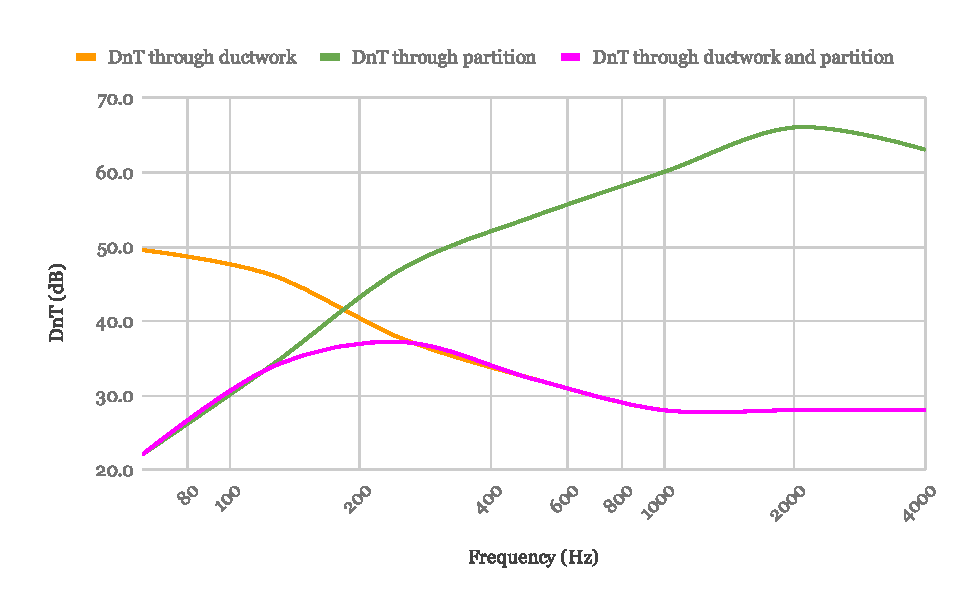
\includegraphics[width=\textwidth]{figures/DnT.eps}
	\rule{\textwidth}{0.5pt} % use line???
	\caption{D\textsubscript{nT} between the conference room and single office for voice transmission through the ductwork and partition.}
	\label{fig:DnT}
\end{figure}



\subsection{Step 2: Calculate D\textsubscript{nT,w}} \label{sec:Q4.2}

The second step is to calculate D\textsubscript{nT,w} through the ductwork, through the partition, and through both the ductwork and the partition.
However, before we can do this, we need to extrapolate the third octave band values of D\textsubscript{nT}.
The extrapolation calculation is demonstrated in Table~\ref{tbl:DnT_extrapolation}.

% Please add the following required packages to your document preamble:
% \usepackage{booktabs}
\begin{table}[htbp]
	\caption{A sample calculation of the extrapolation of the third octave band values of D\textsubscript{nT} through the ductwork.}
	\label{tbl:DnT_extrapolation}
	\centering
	\begin{tabular}{@{}rrl@{}}
		\toprule
		Frequency (Hz) & D\textsubscript{nT} through ductwork (dB) & Notes \\ \midrule
		63 & 50 & From Table~\ref{tbl:DnT} \\
		80 & $50 + \frac{46 - 50}{3} = 48$ &  \\
		100 & $50 + \frac{2 \times (46 - 50)}{3} = 47$ &  \\
		125 & 46 & From Table~\ref{tbl:DnT} \\
		160 & $46 + \frac{38 - 46}{3} = 43$ &  \\
		200 & $46 + \frac{2 \times (38 - 46)}{3} = 40$ &  \\
		250 & 38 & From Table~\ref{tbl:DnT} \\
		\ldots & \ldots & \ldots \\ \bottomrule
	\end{tabular}
\end{table}

Once the third octave band values are calculated, we can calculate D\textsubscript{nT,w}.
This is done by summing the positive differences of a standard curve's D\textsubscript{nT} values minus the measured data's D\textsubscript{nT} values.
The standard curve that gives a sum of differences that is less than or equal to 32~dB (but which is as close as possible to 32~dB) is the D\textsubscript{nT,w}.
Tables~\ref{tbl:DnTw_ductwork}, \ref{tbl:DnTw_partition} and \ref{tbl:DnTw_both} respectively show the calculation of D\textsubscript{nT,w} through the ductwork, through the partition and through both the ductwork and partition.
The highlighted cells in the tables show the sum of differences closest to, yet less than, 32~dB and the corresponding D\textsubscript{nT,w} values.
Subsequently, the D\textsubscript{nT,w} results are:
\begin{itemize}
	\item Through the ductwork only: 29~dB
	\item Through the partition only: 56~dB
	\item Through both the ductwork and partition: 29~dB
\end{itemize}

The charts in Figures~\ref{fig:DnTw_ductwork}, \ref{fig:DnTw_partition} and \ref{fig:DnTw_both} present the D\textsubscript{nT,w} standard curves with the D\textsubscript{nT} data for the ductwork, partition, and both the ductwork and partition, respectively.

% Please add the following required packages to your document preamble:
% \usepackage{booktabs}
\begin{table}[htbp]
	\caption{Calculation of D\textsubscript{nT,w} through the ductwork only.}
	\label{tbl:DnTw_ductwork}
	\centering
	\begin{tabu} to \textwidth {@{}X[r]X[r]X[r]X[r]X[r]X[r]X[r]X[r]X[r]X[r]X[r]X[r]X[r]X[r]@{}}
		\toprule
		Freq (Hz) & D\textsubscript{nT} (dB) & 52 dB Curve & Diff & 42 dB Curve & Diff & 32 dB Curve & Diff & 27 dB Curve & Diff & 28 dB Curve & Diff & \cellcolor{orange} 29 dB Curve & Diff \\ \midrule
		63 & 50 & - & - & - & - & - & - & - & - & - & - & - & - \\
		80 & 48 & - & - & - & - & - & - & - & - & - & - & - & - \\
		100 & 47 & 33 & - & 23 & - & 13 & - & 8 & - & 9 & - & 10 & - \\
		125 & 46 & 36 & - & 26 & - & 16 & - & 11 & - & 12 & - & 13 & - \\
		160 & 43 & 39 & - & 29 & - & 19 & - & 14 & - & 15 & - & 16 & - \\
		200 & 40 & 42 & 2 & 32 & - & 22 & - & 17 & - & 18 & - & 19 & - \\
		250 & 38 & 45 & 7 & 35 & - & 25 & - & 20 & - & 21 & - & 22 & - \\
		315 & 36 & 48 & 12 & 38 & 2 & 28 & - & 23 & - & 24 & - & 25 & - \\
		400 & 34 & 51 & 17 & 41 & 7 & 31 & - & 26 & - & 27 & - & 28 & - \\
		500 & 32 & 52 & 20 & 42 & 10 & 32 & - & 27 & - & 28 & - & 29 & - \\
		630 & 31 & 53 & 22 & 43 & 12 & 33 & 2 & 28 & - & 29 & - & 30 & - \\
		800 & 29 & 54 & 25 & 44 & 15 & 34 & 5 & 29 & - & 30 & 1 & 31 & 2 \\
		1000 & 28 & 55 & 27 & 45 & 17 & 35 & 7 & 30 & 2 & 31 & 3 & 32 & 4 \\
		1250 & 28 & 56 & 28 & 46 & 18 & 36 & 8 & 31 & 3 & 32 & 4 & 33 & 5 \\
		1600 & 28 & 56 & 28 & 46 & 18 & 36 & 8 & 31 & 3 & 32 & 4 & 33 & 5 \\
		2000 & 28 & 56 & 28 & 46 & 18 & 36 & 8 & 31 & 3 & 32 & 4 & 33 & 5 \\
		2500 & 28 & 56 & 28 & 46 & 18 & 36 & 8 & 31 & 3 & 32 & 4 & 33 & 5 \\
		3150 & 28 & 56 & 28 & 46 & 18 & 36 & 8 & 31 & 3 & 32 & 4 & 33 & 5 \\
		4000 & 28 & - & - & - & - & - & - & - & - & - & - & - & - \\ \midrule
		\multicolumn{3}{r}{Sum of differences (dB)} & 271 &  & 153 &  & 54 &  & 17 &  & 23 &  & \cellcolor{orange} 30 \\ \bottomrule
	\end{tabu}
\end{table}

\begin{figure}[htbp]
	\centering
	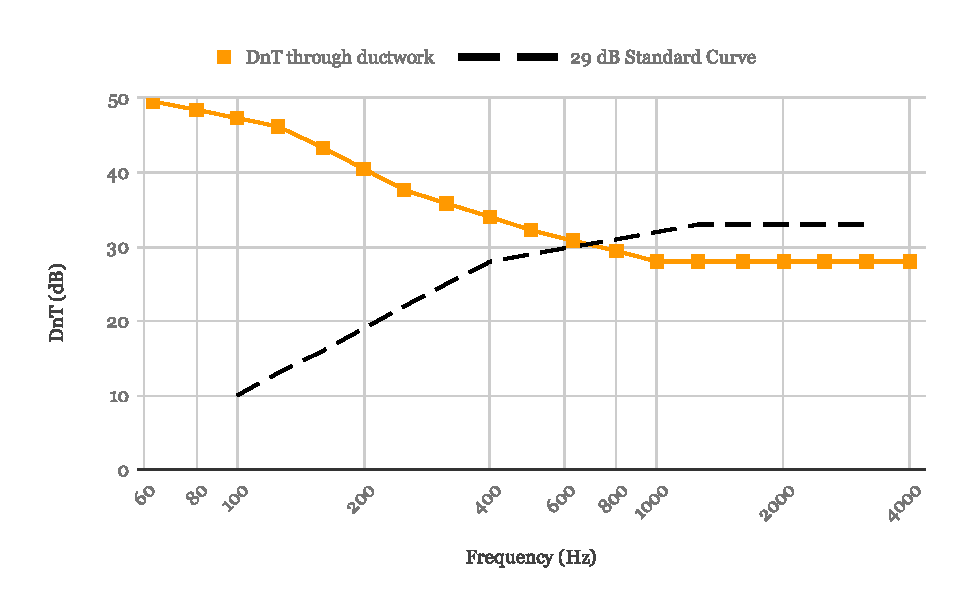
\includegraphics[width=\textwidth]{figures/DnTw_D.eps}
	\rule{\textwidth}{0.5pt} % use line???
	\caption{D\textsubscript{nT} data for the ductwork plotted with the 29~dB standard D\textsubscript{nT,w} curve.}
	\label{fig:DnTw_ductwork}
\end{figure}

% Please add the following required packages to your document preamble:
% \usepackage{booktabs}
\begin{table}[htbp]
	\caption{Calculation of D\textsubscript{nT,w} through the partition only.}
	\label{tbl:DnTw_partition}
	\centering
	\begin{tabular}{@{}rrrrrrrrrr@{}}
		\toprule
		Frequency (Hz) & D\textsubscript{nT} (dB) & 52 dB Curve & Diff & 62 dB Curve & Diff & 57 dB Curve & Diff & \cellcolor{green} 56 dB Curve & Diff \\ \midrule
		63 & 22 & - & - & - & - & - & - & - & - \\
		80 & 26 & - & - & - & - & - & - & - & - \\
		100 & 30 & 33 & 3 & 43 & 13 & 38 & 8 & 37 & 7 \\
		125 & 34 & 36 & 2 & 46 & 12 & 41 & 7 & 40 & 6 \\
		160 & 38 & 39 & 1 & 49 & 11 & 44 & 6 & 43 & 5 \\
		200 & 43 & 42 & - & 52 & 9 & 47 & 4 & 46 & 3 \\
		250 & 47 & 45 & - & 55 & 8 & 50 & 3 & 49 & 2 \\
		315 & 49 & 48 & - & 58 & 9 & 53 & 4 & 52 & 3 \\
		400 & 52 & 51 & - & 61 & 9 & 56 & 4 & 55 & 3 \\
		500 & 54 & 52 & - & 62 & 8 & 57 & 3 & 56 & 2 \\
		630 & 56 & 53 & - & 63 & 7 & 58 & 2 & 57 & 1 \\
		800 & 58 & 54 & - & 64 & 6 & 59 & 1 & 58 & - \\
		1000 & 60 & 55 & - & 65 & 5 & 60 & - & 59 & - \\
		1250 & 62 & 56 & - & 66 & 4 & 61 & - & 60 & - \\
		1600 & 64 & 56 & - & 66 & 2 & 61 & - & 60 & - \\
		2000 & 66 & 56 & - & 66 & - & 61 & - & 60 & - \\
		2500 & 65 & 56 & - & 66 & 1 & 61 & - & 60 & - \\
		3150 & 64 & 56 & - & 66 & 2 & 61 & - & 60 & - \\
		4000 & 63 & - & - & - & - & - & - & - & - \\ \midrule
		\multicolumn{3}{r}{Sum of differences (dB)} & 5 &  & 105 &  & 41 &  & \cellcolor{green} 31 \\ \bottomrule
	\end{tabular}
\end{table}

\begin{figure}[htbp]
	\centering
	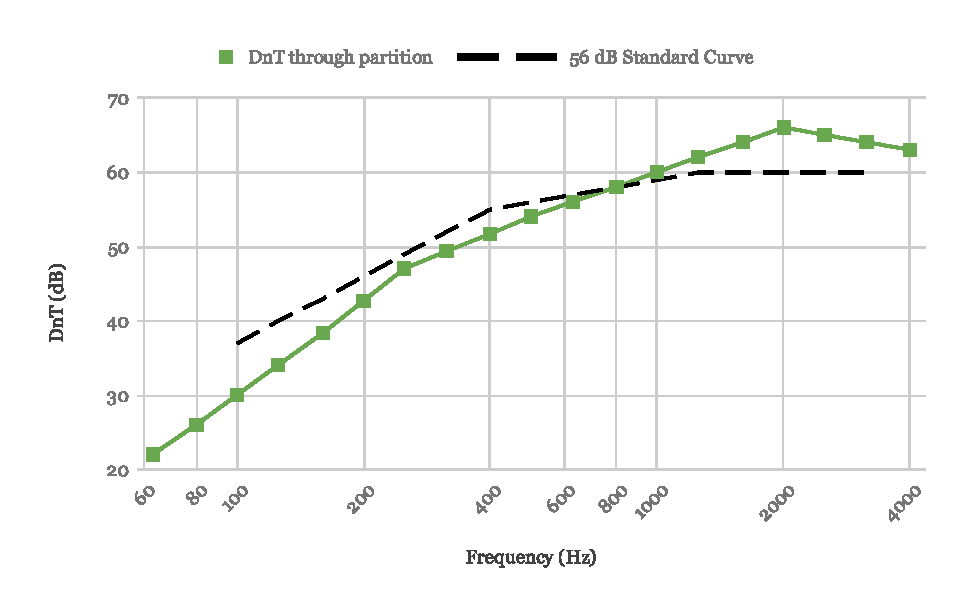
\includegraphics[width=\textwidth]{figures/DnTw_P.eps}
	\rule{\textwidth}{0.5pt} % use line???
	\caption{D\textsubscript{nT} data for the partition plotted with the 56~dB standard D\textsubscript{nT,w} curve.}
	\label{fig:DnTw_partition}
\end{figure}

% Please add the following required packages to your document preamble:
% \usepackage{booktabs}
\begin{table}[htbp]
	\caption{Calculation of D\textsubscript{nT,w} through both the ductwork and partition.}
	\label{tbl:DnT_both}
	\centering
	\begin{tabular}{@{}rrrrrr@{}}
		\toprule
		Frequency (Hz) & D\textsubscript{nT} (dB) & 52 dB Curve & Diff & \cellcolor{yellow} 29 dB Curve & Diff \\ \midrule
		63 & 22 & - & - & - & - \\
		80 & 26 & - & - & - & - \\
		100 & 30 & 33 & 3 & 10 & - \\
		125 & 34 & 36 & 2 & 13 & - \\
		160 & 35 & 39 & 4 & 16 & - \\
		200 & 36 & 42 & 6 & 19 & - \\
		250 & 37 & 45 & 8 & 22 & - \\
		315 & 36 & 48 & 12 & 25 & - \\
		400 & 34 & 51 & 17 & 28 & - \\
		500 & 32 & 52 & 20 & 29 & - \\
		630 & 31 & 53 & 22 & 30 & - \\
		800 & 29 & 54 & 25 & 31 & 2 \\
		1000 & 28 & 55 & 27 & 32 & 4 \\
		1250 & 28 & 56 & 28 & 33 & 5 \\
		1600 & 28 & 56 & 28 & 33 & 5 \\
		2000 & 28 & 56 & 28 & 33 & 5 \\
		2500 & 28 & 56 & 28 & 33 & 5 \\
		3150 & 28 & 56 & 28 & 33 & 5 \\
		4000 & 28 & - & - & - & - \\ \midrule
		\multicolumn{3}{r}{Sum of differences (dB)} & 286 &  & \cellcolor{yellow} 30 \\ \bottomrule
	\end{tabular}
\end{table}

\begin{figure}[htbp]
	\centering
	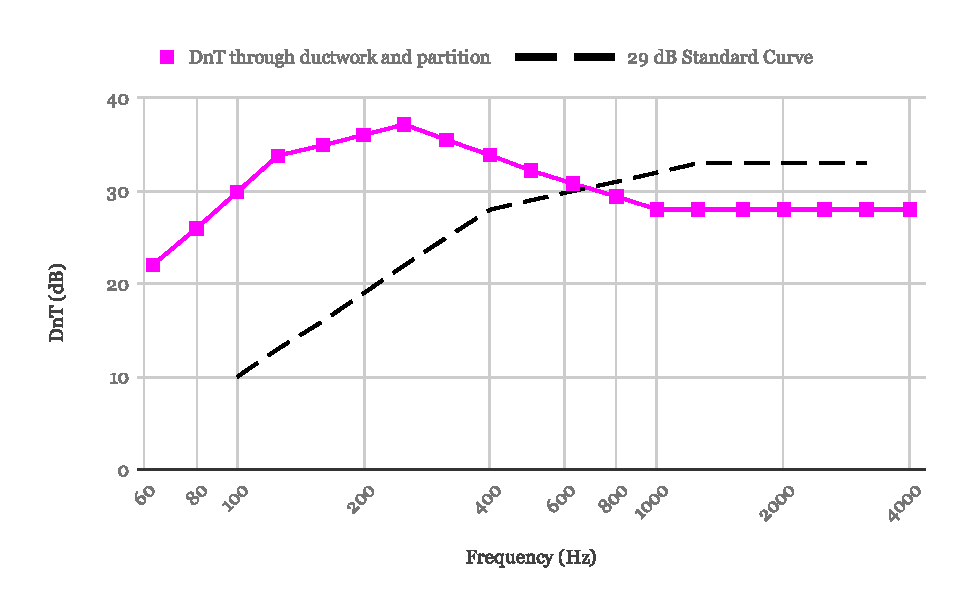
\includegraphics[width=\textwidth]{figures/DnTw_D+P.eps}
	\rule{\textwidth}{0.5pt} % use line???
	\caption{D\textsubscript{nT} data for the ductwork and partition plotted with the 29~dB standard D\textsubscript{nT,w} curve.}
	\label{fig:DnTw_both}
\end{figure}



\newpage
\subsection{Step 3: Calculate the NR value of the single office} \label{sec:Q4.3}

The third step is to calculate the background noise in the single office.
To do this, we first need to calculate the SPL in the office due to fan noise transmitted through the ductwork, L\textsubscript{p\textsubscript{2}}.
As the procedure is very similar to the calculation of L\textsubscript{p\textsubscript{1}} in Question~1 (Section~\ref{sec:Q1}), it will not be explained here.
Table~\ref{tbl:BN_office_example} details the calculation of L\textsubscript{p\textsubscript{2}} at 63~Hz.
Table~\ref{tbl:BN_office} and Figure~\ref{fig:Lp1+2} present the L\textsubscript{p\textsubscript{2}} results in octave bands between 63~Hz and 4~kHz.

% Please add the following required packages to your document preamble:
% \usepackage{booktabs}
\begin{table}[htbp]
	\caption{Calculation of the SPL in the single office due to fan noise, L\textsubscript{p\textsubscript{2}}.}
	\label{tbl:BN_office}
	\centering
	\begin{tabular}{@{}lrrrrrrr@{}}
		\toprule
		Frequency (Hz) & 63 & 125 & 250 & 500 & 1000 & 2000 & 4000 \\ \midrule
		L\textsubscript{W\textsubscript{fan}} (dB re 10\textsuperscript{-12} W) & 92 & 94 & 94 & 93 & 92 & 88 & 84 \\
		Attn\textsubscript{sound attenuator} (dB) & 6 & 9 & 16 & 27 & 31 & 30 & 21 \\
		Attn\textsubscript{horizontal} (dB) & 50.16 & 50.16 & 31.54 & 18.62 & 7.41 & 7.41 & 7.41 \\
		Attn\textsubscript{horizontal $\rightarrow$ vertical} (dB) & 4.77 & 4.77 & 4.77 & 4.77 & 4.77 & 4.77 & 4.77 \\
		Attn\textsubscript{vertical} (dB) & 1.00 & 1.32 & 1.00 & 0.66 & 0.23 & 0.23 & 0.23 \\
		Attn\textsubscript{end reflections} (dB) & 11 & 7 & 3 & 1 & 0 & 0 & 0 \\
		$\Sigma$Attn (dB) & 72.93 & 72.25 & 56.31 & 52.05 & 43.41 & 42.41 & 33.41 \\
		L\textsubscript{W\textsubscript{out}} (dB re 10\textsuperscript{-12} W) & 19.07 & 21.75 & 37.69 & 40.95 & 48.59 & 45.59 & 50.59 \\
		T\textsubscript{2} (s) & 0.47 & 0.41 & 0.46 & 0.48 & 0.36 & 0.31 & 0.30 \\
		SPL in single office due to single ductwork, L\textsubscript{p\textsubscript{2 single}} (dB) & 12.79 & 14.87 & 31.29 & 34.75 & 41.18 & 37.54 & 42.34 \\
		SPL in single office due to supply and return, L\textsubscript{p\textsubscript{2}} (dB) & 15.8 & 17.9 & 34.3 & 37.8 & 44.2 & 40.5 & 45.3 \\ \bottomrule
	\end{tabular}
\end{table}

\begin{figure}[H]
	\centering
	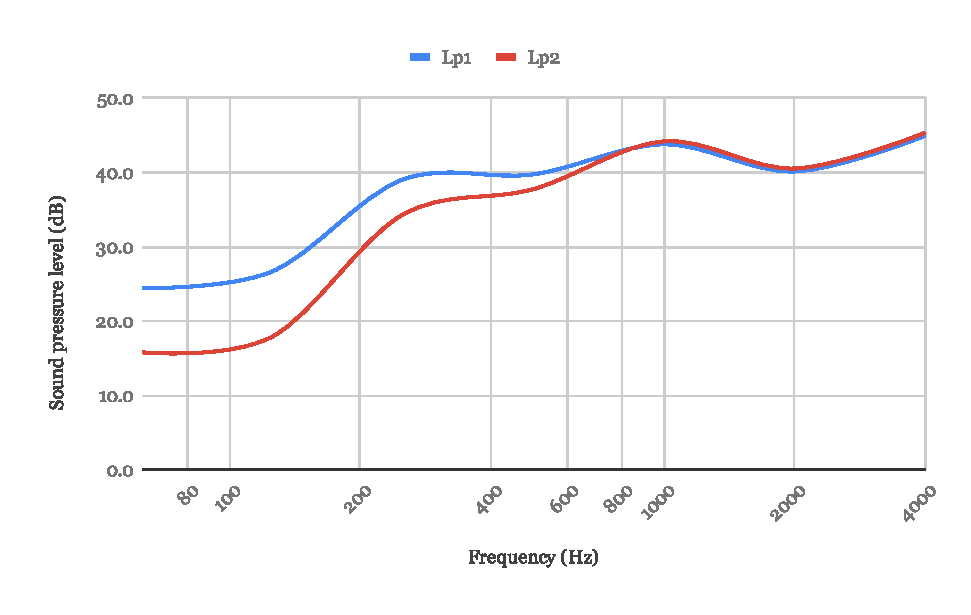
\includegraphics[width=\textwidth]{figures/Lp1+2.eps}
	\rule{\textwidth}{0.5pt} % use line???
	\caption{The SPLs due to fan noise transmitted through the ductwork (both supply and return) in the conference room, L\textsubscript{p\textsubscript{1}}, and the single office, L\textsubscript{p\textsubscript{2}}.}
	\label{fig:Lp1+2}
\end{figure}

% Please add the following required packages to your document preamble:
% \usepackage{booktabs}
\begin{sidewaystable}[htbp]
	\caption{Details of the calculation of the SPL in the conference room due to fan noise, L\textsubscript{p\textsubscript{2}}, at 63~Hz.}
	\label{tbl:BN_office_example}
	\centering
	\begin{tabular}{@{}m{5cm}rm{12cm}@{}}
		\toprule
		Frequency (Hz) & 63 & Notes \\ \midrule
		L\textsubscript{W\textsubscript{fan}} (dB re 10\textsuperscript{-12} W) & 92 & Given in Table~1 of assignment description \\
		& \multicolumn{1}{l}{} &  \\
		Attn\textsubscript{sound attenuator} (dB) & 6 & Given in Table~5 of assignment description \\
		& \multicolumn{1}{l}{} &  \\
		Attn\textsubscript{horizontal} (dB) & $19 \times (1 + 1.64) = 50.16$ & Same as notes for Attn\textsubscript{horizontal} in Table~\ref{tbl:BN_conf_example}, but for a duct length of 19~m \\
		& \multicolumn{1}{l}{} &  \\
		Attn\textsubscript{horizontal $\rightarrow$ vertical} (dB) & $\left|10 log \frac{0.12}{0.12 + 0.24}\right| = 4.77$ & $\left|10 log \frac{S_{vertical}}{S_{vertical} + S_{horizontal}}\right|$ \\
		& \multicolumn{1}{l}{} &  \\
		Attn\textsubscript{vertical} (dB) & $0.5 \times (1 + 1) = 1.00$ & Same as notes for Attn\textsubscript{vertical} in Table~\ref{tbl:BN_conf_example} \\
		& \multicolumn{1}{l}{} &  \\
		Attn\textsubscript{end reflections} (dB) & 11 & Given in Table~6 of assignment description for a duct cross-sectional area of 0.3~m $\times$ 0.4~m = 0.12~m\textsuperscript{2} \\
		& \multicolumn{1}{l}{} &  \\
		$\Sigma$Attn (dB) & 72.93 & Sum of all attenuations \\
		& \multicolumn{1}{l}{} &  \\
		L\textsubscript{W\textsubscript{out}} (dB re 10\textsuperscript{-12} W) & $92 - 72.93 = 19.07$ & Sound power level leaving single ductwork: $L_{W out} = L_{W fan} - \Sigma Attn$ \\
		& \multicolumn{1}{l}{} &  \\
		T\textsubscript{2} (s) & 0.47 & From Table~\ref{tbl:reverb_office} \\
		& \multicolumn{1}{l}{} &  \\
		SPL in single office due to single ductwork, L\textsubscript{p\textsubscript{2 single}} (dB) & $19.07 - 10 log \frac{50}{0.47} + 14 = 12.79$ & $L_{p_2 single} = L_{W out} – 10 log \frac{V_2}{T_{2}} + 14$ \\
		& \multicolumn{1}{l}{} &  \\
		SPL in single office due to supply and return, L\textsubscript{p\textsubscript{2}} (dB) & $12.79 + 3 = 15.8$ & Sum of two identical SPLs = $L_p + 3$ \\ \bottomrule
	\end{tabular}
\end{sidewaystable}

Afterwards, the L\textsubscript{p\textsubscript{2}} values are plotted onto an NR curve chart to find the office's NR value, much like in Question~2 (Section~\ref{sec:Q2}).
As seen in Figure~\ref{fig:NR_office}, the SPLs lie on/ below the NR 50 curve.
Therefore, the single office's noise rating is NR 50.

\begin{figure}[htbp]
	\centering
	\includegraphics[height=.72\textheight]{figures/NR_office.jpg}
	\rule{.6\textwidth}{0.5pt} % use line???
	\caption{The NR of the single office.}
	\label{fig:NR_office}
\end{figure}



\newpage
\subsection{Conversation privacy} \label{sec:Q4.4}

By summing the D\textsubscript{nT,w} results with the NR rating of the single office, one can deduce whether the conversation with a raised male voice in the conference room can be overheard in the single office.
Table~\ref{tbl:privacy_criteria} gives the criteria for conversation privacy and Table~\ref{tbl:privacy} presents the sums of D\textsubscript{nT,w} and NR.

As seen in Table~\ref{tbl:privacy}, the conference room conversation is completely inaudible from the single office when you just consider sound transmission through the partition ($D\textsubscript{nT,w} + NR = 106~dB$).
However, when you consider sound transmission through the ductwork and both the ductwork and partition, the conference room conversation is faintly audible but not intelligible from the single office ($D\textsubscript{nT,w} + NR = 79~dB$).
These results can be interpreted as follows:
the partition has enough \textbf{\textit{absorption}} to guarantee privacy in the conference room. 
The only sound one can overhear from the single office comes through the ductwork.
That is why the ductwork only and ductwork + partition results are the same (i.e. audible but not intelligible).

% Please add the following required packages to your document preamble:
% \usepackage{booktabs}
\begin{table}[htbp]
	\caption{Conversation privacy criteria \citep{unit6}.}
	\label{tbl:privacy_criteria}
	\centering
	\begin{tabular}{@{}lc@{}}
		\toprule
		Sound as heard by occupant & D\textsubscript{w} + NR (dB) \\ \midrule
		Intelligible & $< 60$ \\
		Occasionally intelligible & $60 - 70$ \\
		Audible but not intelligible & $70 - 80$ \\
		Inaudible & $> 80$ \\ \bottomrule
	\end{tabular}
\end{table}

% Please add the following required packages to your document preamble:
% \usepackage{booktabs}
\begin{table}[htbp]
	\caption{Privacy of the conversation in the conference room as overheard from the single office.}
	\label{tbl:privacy}
	\centering
	\begin{tabular}{@{}lrrrl@{}}
		\toprule
		& D\textsubscript{nT,w} (dB) & NR (dB) & D\textsubscript{nT,w} + NR (dB) & Sound as heard by office occupant \\ \midrule
		 Ductwork & 29 & 50 & 79 & Audible but not intelligible \\
		 Partition & 56 & 50 & 106 & Inaudible \\
		 Ductwork and partition & 29 & 50 & 79 & Audible but not intelligible \\ \bottomrule
	\end{tabular}
\end{table}